\documentclass[11pt]{scrartcl}

\usepackage[sexy]{evan}
\usepackage{pgfplots}
\pgfplotsset{compat=1.15}
\usepackage{mathrsfs}
\usetikzlibrary{arrows}
\usepackage{graphics}
\usepackage{tikz}
\usepackage{ amssymb }
\usepackage[dvipsnames]{xcolor}
\usepackage[utf8]{inputenc}
\usepackage{longtable}
\usepackage{ragged2e}
\usepackage{listings}
\definecolor{red1}{RGB}{255, 153, 153}
\definecolor{green1}{RGB}{204, 255, 204}
\definecolor{blue1}{RGB}{204, 255, 255}
\definecolor{yellow1}{RGB}{255, 247, 160}

\definecolor{red2}{RGB}{255, 102, 102}
\definecolor{green2}{RGB}{108, 255, 108}
\definecolor{blue2}{RGB}{94, 204, 255}
\definecolor{yellow2}{RGB}{255, 250, 104}

\definecolor{red2.5}{RGB}{255,76,76}
\definecolor{green2.5}{RGB}{54, 247, 54}
\definecolor{blue2.5}{RGB}{51, 189, 255}
\definecolor{yellow2.5}{RGB}{255, 242, 52}


\definecolor{red3}{RGB}{255, 51, 51}
\definecolor{green3}{RGB}{0, 240, 0}
\definecolor{blue3}{RGB}{9, 175, 255}
\definecolor{yellow3}{RGB}{255, 234, 0}

\definecolor{red3.5}{RGB}{229, 25, 25}
\definecolor{green3.5}{RGB}{0, 194, 0}
\definecolor{blue3.5}{RGB}{4, 143, 209}
\definecolor{yellow3.5}{RGB}{255,220,0}

\definecolor{red4}{RGB}{204, 0, 0}
\definecolor{green4}{RGB}{0, 149, 0}
\definecolor{blue4}{RGB}{0, 111, 164}
\definecolor{yellow4}{RGB}{255, 206, 0}


\definecolor{noseve}{RGB}{242,242,242}

\newcommand{\camod}[1]{\frac{\ZZ}{#1 \ZZ}}
\newcommand{\modm}[1]{\text{ mod } #1}
\newcommand{\campm}[1]{\frac{\ZZ}{m\ZZ}}

\usepackage{epigraph}
\renewcommand{\epigraphsize}{\scriptsize}
\renewcommand{\epigraphwidth}{60ex}


\definecolor{dcol0}{HTML}{C8E6C9}
\definecolor{dcol1}{HTML}{D4E9B3}
\definecolor{dcol2}{HTML}{E5ED9A}
\definecolor{dcol3}{HTML}{FFF59D}
\definecolor{dcol4}{HTML}{FFE082}
\definecolor{dcol5}{HTML}{FFCC80}
\definecolor{dcol6}{HTML}{FFAB91}
\definecolor{dcol7}{HTML}{F49890}
\definecolor{dcol8}{HTML}{E57373}
\definecolor{dcol9}{HTML}{D32F2F}

\makeatletter
\newcommand{\getcolorname}[1]{dcol#1}
\makeatother

\newcommand{\dif}[1]{%
    \edef\colorindex{\number\fpeval{floor(#1)}}%
    \edef\fulltext{#1}%
    \colorbox{\getcolorname{\colorindex}}{%
        \ifnum\colorindex>8
            \textbf{\textcolor{white}{\,\fulltext\,}}%
        \else
            \textbf{\textcolor{black}{\,\fulltext\,}}%
        \fi
    }%
}
% Variable para dificultad (inicial 0)
\newcommand{\thmdifficulty}{0}

% Comando para asignar dificultad antes del problema
\newcommand{\problemdiff}[1]{\renewcommand{\thmdifficulty}{#1}}

% Estilo del problema que incluye dificultad antes del título
\declaretheoremstyle[
    headfont=\color{blue!40!black}\normalfont\bfseries,
    headformat={%
      \dif{\thmdifficulty}\quad \NAME~\NUMBER\ifx\relax\EMPTY\relax\else\ \NOTE\fi
    },
    postheadspace=1em,
    spaceabove=8pt,
    spacebelow=8pt,
    bodyfont=\normalfont
]{problemstyle}

    \declaretheorem[style=problemstyle,name=Problema,sibling=theorem]{problema}
    \declaretheorem[style=problemstyle,name=Problema,numbered=no]{problema*}

\title {7.- Maqueta (Practica 1)}
\subtitle{Programación WEB I \\ Centro de Enseñanza Tecnica Industrial}
\date{1 de Octubre de 2025}
\author{Emmanuel Buenrostro 22300891 7F1}


\begin{document}

\maketitle


\begin{center}
   
\includegraphics[scale=0.15]{../cetilogo.jpg} 
\end{center}
\newpage
\tableofcontents


\section{Resumen}

Hice un CV en HTML y CSS, el cual esta dividido en tres partes, para eso esta acomodado por divs, además de sus respectivos Wireframe y Prototipo.

\section{Objetivo}
Crear la maqueta (estructura HTML con su respectivo CSS) donde se muestre tu curriculum vitae orientado a desarrollo de software

\section{Diagramas}
\subsection{Wireframe}
\begin{center}
    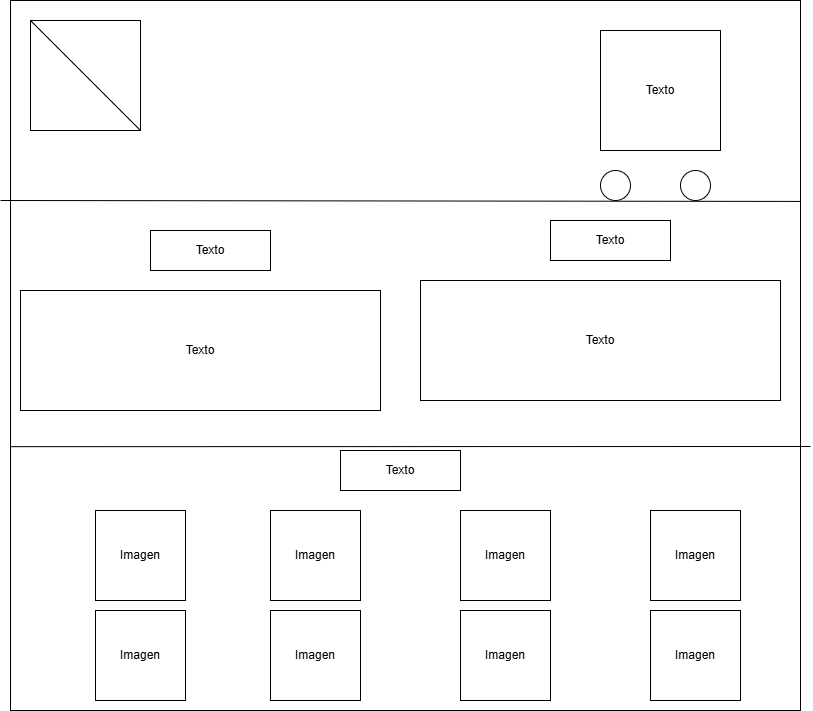
\includegraphics[scale=0.6]{wireframe.png}
\end{center}

\subsection{Prototipo}
\begin{center}
    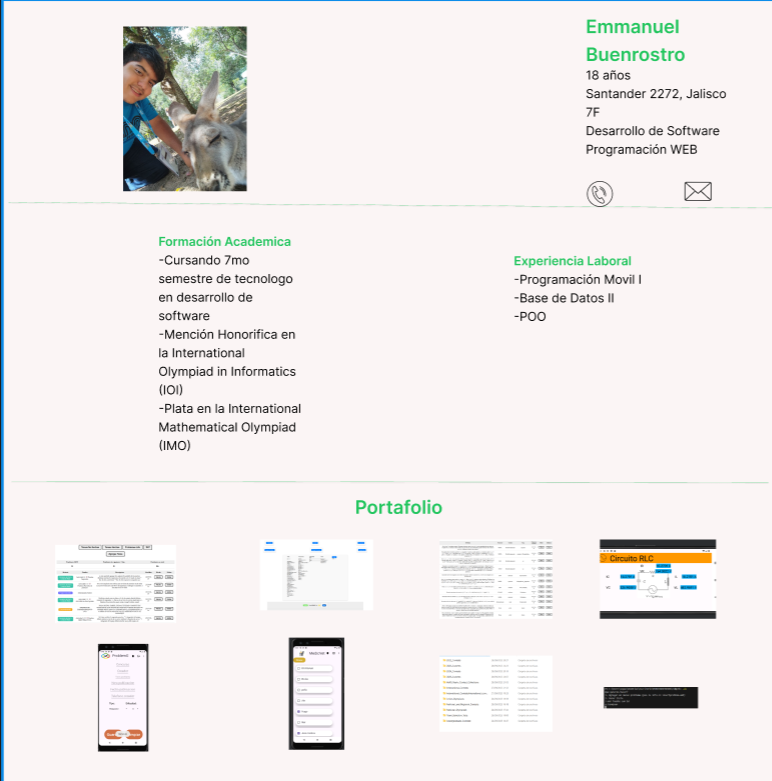
\includegraphics[scale=0.8]{Maquetado.png}
\end{center}

\section{Codigo}

\subsection{HTML}
\lstinputlisting[language=html]{index.html}

\subsection{CSS}
\lstinputlisting{styles.css}

\section{Evidencia}

\begin{center}
    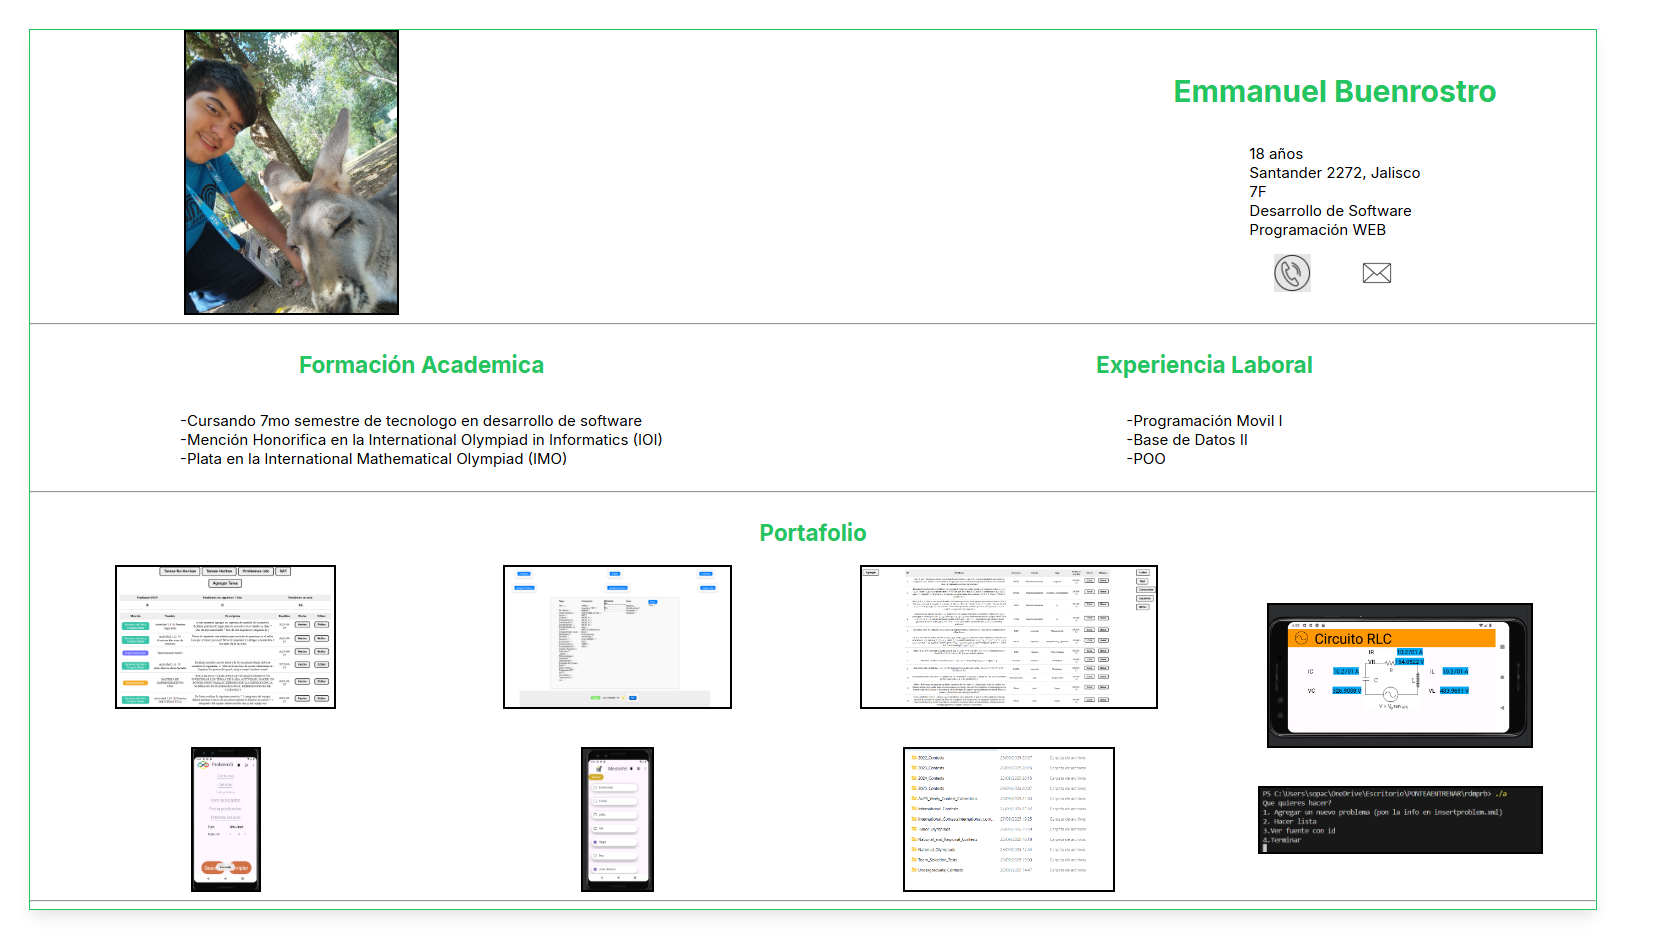
\includegraphics[scale=0.4]{Pagina.png}
\end{center}

\subsection{Justificación}

Se uso un fondo blanco algo amarillo para que se vea claro pero no cale a la vista. La información de los textos es negra para que resalte con el fondo. Para remarcar cosas como mi nombre use el color verde, ya que este si reslta con el fondo y además suele ser usado como positivo. 
Se usa la tipografia Inter ya que se ve muy bien en pantallas y es facil de leer.

\section{Conclusión}

Logre hacer una pagina donde usamos los conocimientos de CSS y HTML que hemos adquirido, asi como acomodarla por divs para que este de una forma mas clara, 
y el uso de class e id para dar atributos especificos en CSS, asi como dar atributos a todas las etiquetas de un tipo como h1.

    \end{document}